\documentclass[11pt,letterpaper]{article}

\usepackage[spanish,es-nosectiondot]{babel}
\usepackage[utf8]{inputenc}
\usepackage[T1]{fontenc}
\usepackage{amsmath}
\usepackage{booktabs}
\usepackage{caption}
\usepackage{float}
\usepackage{geometry}
\usepackage{graphicx}
\usepackage{longtable}
\usepackage{pdflscape}
\usepackage{array}
\usepackage{tabularx}
\usepackage{threeparttable}
\usepackage{xurl}

\geometry{margin=2.5cm}

\graphicspath{{../../../02_eda/eda_qr_vs_bip_profiles_files/figure-html/}{figures/}}

\title{EDA QR vs BIP: patrones descriptivos e interanuales}
\author{Juan Vicente Onetto Romero}
\date{Julio 2026}

\begin{document}

\maketitle

\section{Objetivo y lectura general}

Este reporte resume los principales resultados del EDA QR vs BIP. El objetivo no
es documentar todo el notebook, sino dejar una lectura breve y visual sobre tres
preguntas: en qué se diferencia QR de BIP, qué parte de esa diferencia parece
territorial o contextual, y cómo cambia el uso QR entre 2024 y 2025.

La unidad principal del EDA es la tarjeta observada, no una persona única. Por
eso, las diferencias se interpretan como diferencias entre tarjetas o
poblaciones observadas. En el bloque interanual, la unidad cambia a ZONA777 para
comparar el share QR entre ventanas equivalentes de 2024 y 2025. En ambos casos,
la lectura es descriptiva y no causal.

La lectura central es que QR no aparece como una versión idéntica de BIP. Es un
medio de pago minoritario, menos intensivo y menos regular, con mayor presencia
relativa en 2025. Territorialmente, QR se asocia más con zonas de mayor educación
residencial, mayor centralidad urbana y mayor presencia Metro. En cambio, no hay
evidencia clara de que el crecimiento QR se explique principalmente por peor
acceso físico a carga BIP.

\begin{table}[H]
\centering
\caption{Lectura general del EDA}
\small
\setlength{\tabcolsep}{5pt}
\renewcommand{\arraystretch}{1.22}
\begin{tabularx}{\textwidth}{>{\raggedright\arraybackslash}p{4.0cm} >{\raggedright\arraybackslash}X}
\toprule
Eje & Resultado principal \\
\midrule
Composición & QR representa 15.3\% de las tarjetas y 13.6\% de los viajes observados. Su peso es menor en viajes que en tarjetas. \\
Uso & QR tiene menos viajes y menos días activos por tarjeta. La diferencia en semanas activas es más débil. \\
Perfil temporal y modal & QR muestra una señal algo más desplazada hacia horarios no laborales, fines de semana y viajes unimodales. No es una separación radical. \\
Territorio y residencia & QR pesa más en zonas asociadas a mayor educación, mayor ingreso residencial y mayor presencia de población adulta joven. \\
Contexto urbano y operacional & Las señales OSM y operacionales describen centralidad y contexto urbano. QR aparece más asociado a presencia Metro que a entornos bus densos o con alta relación demanda-oferta. \\
Cambio interanual & Entre ventanas equivalentes 2024--2025, QR crece casi en todas las zonas comparables. La geografía previa se mantiene y, en parte, se refuerza. \\
\bottomrule
\end{tabularx}
\end{table}

El reporte usa gráficos como evidencia principal y texto breve para orientar la
lectura. Las figuras del cuerpo muestran los patrones más comunicables; las
figuras de auditoría, sensibilidad o lectura secundaria quedan reservadas para
anexos.

\section{QR es minoritario y menos intensivo}

\subsection{Composición y cohorte temporal}

QR representa una fracción minoritaria del sistema observado. En el periodo de
análisis, alcanza 15.3\% de las tarjetas y 13.6\% de los viajes. La diferencia
entre ambas proporciones es importante: QR pesa menos cuando se mide por viajes
que cuando se mide por tarjetas, lo que anticipa una menor intensidad promedio
de uso.

\begin{figure}[H]
\centering
\includegraphics[width=0.88\textwidth]{block1-composition-plot-output-2.png}
\caption{Composición BIP vs QR en tarjetas y viajes}
\end{figure}

La composición temporal también está desplazada hacia 2025. Entre las tarjetas
QR, 41.3\% aparece solo en 2025, frente a 33.9\% en BIP. Esto no prueba adopción
individual ni reemplazo de BIP por QR, pero sí muestra que QR tiene una presencia
más reciente en la ventana observada.

\begin{figure}[H]
\centering
\includegraphics[width=0.88\textwidth]{block2-cohort-plot-output-2.png}
\caption{Cohorte temporal por medio de pago}
\end{figure}

\subsection{Intensidad de uso}

La menor intensidad QR aparece en las medidas centrales de uso. La mediana de
viajes por tarjeta es 8 en QR y 11 en BIP; la mediana de días activos es 5 en QR
y 6 en BIP. En semanas activas, en cambio, ambos grupos tienen mediana 3. La
brecha principal no está en cuántas semanas aparece una tarjeta, sino en cuántos
viajes y días de uso acumula dentro del periodo observado.

\begin{figure}[H]
\centering
\includegraphics[width=0.88\textwidth]{block3-intensity-plot-output-2.png}
\caption{Intensidad mediana de uso por medio de pago}
\end{figure}

La lectura no depende solo de la mediana. En la figura siguiente, los percentiles
se calculan sobre tarjetas dentro de cada medio de pago: p50 es la mediana del
grupo y p90 deja bajo sí al 90\% de las tarjetas. QR queda por debajo de BIP en
viajes y días activos; en semanas activas, la diferencia es más acotada y aparece
sobre todo en la cola alta.

\begin{figure}[H]
\centering
\includegraphics[width=0.88\textwidth]{block3-intensity-percentile-profile-output-2.png}
\caption{Percentiles de intensidad por tarjeta, calculados dentro de cada medio de pago}
\end{figure}

\subsection{Regularidad y concentración}

La regularidad confirma la misma idea. QR aparece en menos días activos que BIP,
pero cuando aparece no concentra muchos más viajes por día activo. En ambas
tarjetas, la mediana de viajes por día activo es 2. La diferencia principal está
en la frecuencia de aparición, no en una concentración diaria excepcional.

\begin{figure}[H]
\centering
\includegraphics[width=0.88\textwidth]{block4-regularity-raincloud-output-2.png}
\caption{Regularidad temporal y concentración diaria de viajes}
\end{figure}

En síntesis, QR es minoritario, más reciente y menos intensivo que BIP. Esta es
una diferencia entre grupos, no una regla para clasificar tarjetas individuales:
también hay tarjetas BIP de baja intensidad y tarjetas QR con uso frecuente. La
lectura correcta es que la distribución QR se desplaza hacia menor intensidad,
pero no se separa completamente de la distribución BIP.

\section{QR tiene diferencias de uso, pero no radicales}

\subsection{Horario}

Las tarjetas QR no aparecen en un horario completamente distinto a BIP. Ambas
mantienen la estructura general del día, con punta de mañana, valle laboral y
punta de tarde. La diferencia es de énfasis: QR pesa algo más en puntas, horarios
no laborales y viajes más tardíos, mientras BIP mantiene mayor presencia en el
valle laboral.

\begin{figure}[H]
\centering
\includegraphics[width=0.90\textwidth]{block5-timing-share-dumbbells-output-2.png}
\caption{Composición de franjas horarias por medio de pago}
\end{figure}

La brecha más clara está en el valle laboral: QR tiene 51.0\% de sus viajes en
esa franja, frente a 55.7\% en BIP. En cambio, QR queda algo por encima en punta
mañana laboral, punta tarde laboral y horarios no laborales. La lectura es
consistente con un uso QR menos laboral-recurrente, pero no con dos calendarios
horarios separados.

\subsection{Día de semana}

El perfil semanal también es parecido entre medios de pago. Ambos concentran
viajes en días laborales y reducen su peso durante el fin de semana. QR muestra
una participación levemente mayor en sábado y domingo, pero la diferencia es
acotada.

\begin{figure}[H]
\centering
\includegraphics[width=0.90\textwidth]{block6-weekday-plot-output-2.png}
\caption{Distribución semanal BIP vs QR}
\end{figure}

La diferencia semanal refuerza la lectura de regularidad. QR aparece
relativamente menos en días laborales y se acerca más a BIP durante el fin de
semana. No obstante, el patrón general sigue siendo común: QR no se transforma
en un medio principalmente de fin de semana.

\subsection{Perfil modal}

La diferencia modal más comunicable es que QR no aparece más intermodal que BIP.
La señal va en sentido opuesto: QR se asocia levemente más a viajes unimodales y
menos a viajes que combinan Metro y bus dentro del mismo viaje.

\begin{figure}[H]
\centering
\includegraphics[width=0.90\textwidth]{block7-modal-butterfly-output-2.png}
\caption{Perfil modal por medio de pago}
\end{figure}

En promedio por tarjeta, QR tiene mayor peso en solo bus y solo Metro, y menor
peso en la combinación Metro+bus. La brecha más visible está en los viajes
Metro+bus: 13.2\% en QR versus 16.3\% en BIP. Esta diferencia no debe leerse
como preferencia causal por modos simples; puede reflejar diferencias de origen,
acceso a Metro, tipo de viaje o composición de usuarios.

En síntesis, QR muestra diferencias de uso, pero no una ruptura completa con
BIP. Las señales temporales y modales apuntan en una dirección coherente:
menor regularidad laboral, algo más de uso no laboral y menor intermodalidad.
La magnitud, sin embargo, es moderada.

\section{QR tiene una señal territorial y residencial}

\subsection{Geografía de residencia y origen}

La diferencia QR/BIP también tiene estructura territorial. Se observan dos
geografías: la zona de residencia inferida de la tarjeta y la zona donde suele
iniciar viajes. La primera aproxima el entorno residencial; la segunda aproxima
el contexto habitual de uso del sistema. Ambas son descriptivas y no deben
interpretarse como residencia individual observada con certeza ni como causalidad
territorial.

\begin{figure}[H]
\centering
\includegraphics[width=0.94\textwidth]{block8-territorial-macrozone-plot-output-2.png}
\caption{Share QR por macrozona de residencia y origen habitual}
\end{figure}

A nivel de macrozona, QR aparece por sobre su promedio global en Centro y
Oriente, especialmente en residencia. En cambio, Sur y Poniente quedan
consistentemente por debajo. La señal no depende de una sola geografía: residencia
y origen habitual entregan una lectura parecida, aunque no idéntica.

\begin{figure}[H]
\centering
\includegraphics[width=0.92\textwidth]{block8-residence-map-min500-output-2.png}
\caption{Share QR por zona de residencia}
\end{figure}

\begin{figure}[H]
\centering
\includegraphics[width=0.92\textwidth]{block8-origin-map-min500-output-2.png}
\caption{Share QR por zona de origen habitual}
\end{figure}

Los mapas muestran heterogeneidad local dentro de las macrozonas. Aun así, la
lectura general se mantiene: mayor presencia relativa QR en zonas centro-oriente
y menor presencia relativa en varias zonas del sur y poniente. Esto justifica
mirar variables residenciales y de contexto urbano, porque la diferencia no es
solo de intensidad de uso.

\subsection{Ingreso y educación residencial}

Las variables residenciales son atributos de la zona hogar, no de la persona
usuaria. En ingreso se usan proxies territoriales de la EOD 2012; en educación,
el porcentaje de población 18+ con educación universitaria o superior del Censo
2024. Por lo tanto, la lectura es ecológica: describe el entorno residencial
asociado a la tarjeta.

\begin{figure}[H]
\centering
\includegraphics[width=0.92\textwidth]{block9-sociodemographic-raincloud-output-2.png}
\caption{Composición socioeconómica residencial por medio de pago}
\end{figure}

Considerando la clasificación socioeconómica usada en el proxy EOD 2012, D+E
representa hogares de menor nivel socioeconómico y ABC1 representa hogares de
mayor nivel socioeconómico. Con esa definición, QR aparece relativamente menos
asociado a zonas con alta concentración D+E y algo más asociado a zonas con
mayor concentración ABC1. La mediana D+E es 43.7\% en QR versus 46.7\% en BIP;
la mediana ABC1 es 4.9\% en QR versus 4.0\% en BIP. La diferencia no separa
completamente los grupos, pero desplaza a QR hacia zonas residenciales de mayor
nivel socioeconómico.

\begin{figure}[H]
\centering
\includegraphics[width=0.88\textwidth]{block9-sociodemographic-raincloud-output-3.png}
\caption{Ranking de ingreso mediano residencial por medio de pago}
\end{figure}

El ranking de ingreso histórico resume la misma señal: la tarjeta QR mediana
queda en el percentil 56 de ingreso residencial, mientras la tarjeta BIP mediana
queda en el percentil 51. Aquí el percentil también es zonal: cada ZONA777 se
ordena según su ingreso mediano histórico EOD 2012 y cada tarjeta hereda el
percentil de su zona de residencia. Si se agrupa en quintiles, Q1 corresponde a
zonas de menor ingreso residencial relativo y Q5 a zonas de mayor ingreso
residencial relativo. Es una diferencia moderada, pero consistente con la
lectura territorial.

\begin{figure}[H]
\centering
\includegraphics[width=0.82\textwidth]{block9-education-quintile-plot-output-2.png}
\caption{Adopción QR por quintil zonal de educación universitaria residencial}
\end{figure}

Para este gráfico, primero se ordenan las zonas ZONA777 según el porcentaje de
población 18+ con educación universitaria o superior en Censo 2024. Ese ranking
zonal se divide en cinco grupos: Q1 contiene las zonas con menor presencia
universitaria residencial y Q5 las zonas con mayor presencia. Luego cada tarjeta
hereda el quintil de su zona de residencia y se calcula el share QR entre las
tarjetas que caen en cada grupo de zonas.

Con esa definición, la educación residencial entrega el gradiente más claro del
bloque. El share QR sube desde 12.9\% en los quintiles de menor educación
universitaria residencial a 17.9\% en el quintil más alto. Esta señal será
importante para el modelo posterior, porque aparece de forma consistente en
varias lecturas del EDA.

\subsection{Edad residencial}

La composición etaria apunta en una dirección complementaria. QR no se diferencia
mucho en zonas 18--24, probablemente porque parte de la población estudiantil
joven usa TNE y queda clasificada dentro de BIP. La diferencia aparece más en el
ciclo adulto-laboral y en zonas envejecidas.

\begin{figure}[H]
\centering
\includegraphics[width=0.82\textwidth]{block9-age-median-dumbbell-output-2.png}
\caption{Composición etaria residencial por medio de pago}
\end{figure}

QR reside en zonas con mayor presencia de población 25--44 y menor presencia de
población 60+. La diferencia es moderada: 31.8\% versus 30.4\% en 25--44, y
18.8\% versus 20.0\% en 60+. La lectura correcta no es edad individual, sino
contexto residencial de ciclo de vida.

\subsection{Acceso físico a carga BIP}

El acceso a carga BIP se usa como contraste frente a una hipótesis simple: si QR
sustituyera principalmente la fricción de cargar saldo, debería aparecer más en
zonas con peor acceso físico a puntos BIP. Con las variables zonales disponibles,
esa señal no aparece con fuerza.

\begin{figure}[H]
\centering
\includegraphics[width=0.94\textwidth]{block10-bip-load-median-dumbbell-output-2.png}
\caption{Acceso físico a carga BIP por medio de pago}
\end{figure}

Las medianas de distancia al punto de carga más cercano y de densidad de puntos
BIP son muy parecidas entre QR y BIP, tanto en residencia como en origen y
actividad habitual. Esto debilita la hipótesis de que QR se concentre
principalmente donde cargar BIP es territorialmente más difícil.

\begin{figure}[H]
\centering
\includegraphics[width=0.94\textwidth]{block10-bip-load-quintile-plots-output-2.png}
\caption{Adopción QR por distancia a puntos de carga BIP}
\end{figure}

\begin{figure}[H]
\centering
\includegraphics[width=0.94\textwidth]{block10-bip-load-quintile-plots-output-3.png}
\caption{Adopción QR por densidad de puntos de carga BIP}
\end{figure}

Los quintiles refuerzan la misma conclusión. QR no aumenta de forma monotónica
cuando crece la distancia a puntos de carga ni cae de forma clara cuando aumenta
la densidad de carga. Esto no descarta efectos para subgrupos o viajes
específicos, pero a escala ZONA777 el acceso físico a carga BIP no aparece como
el principal organizador territorial de QR.

\section{Contexto urbano y operacional}

\subsection{Centralidad urbana aproximada con OSM}

OpenStreetMap se usa como fuente auxiliar para describir objetos registrados en
el territorio. No mide bancarización individual, acceso digital, calidad de
servicios ni uso efectivo de comercios o equipamientos. Las variables se
construyen como densidades por km2 a escala ZONA777 y se transforman con
\texttt{log1p}, winsorización p99.5 y z-score zonal, para reducir colas largas y
hacer comparables componentes con escalas distintas.

\begin{figure}[H]
\centering
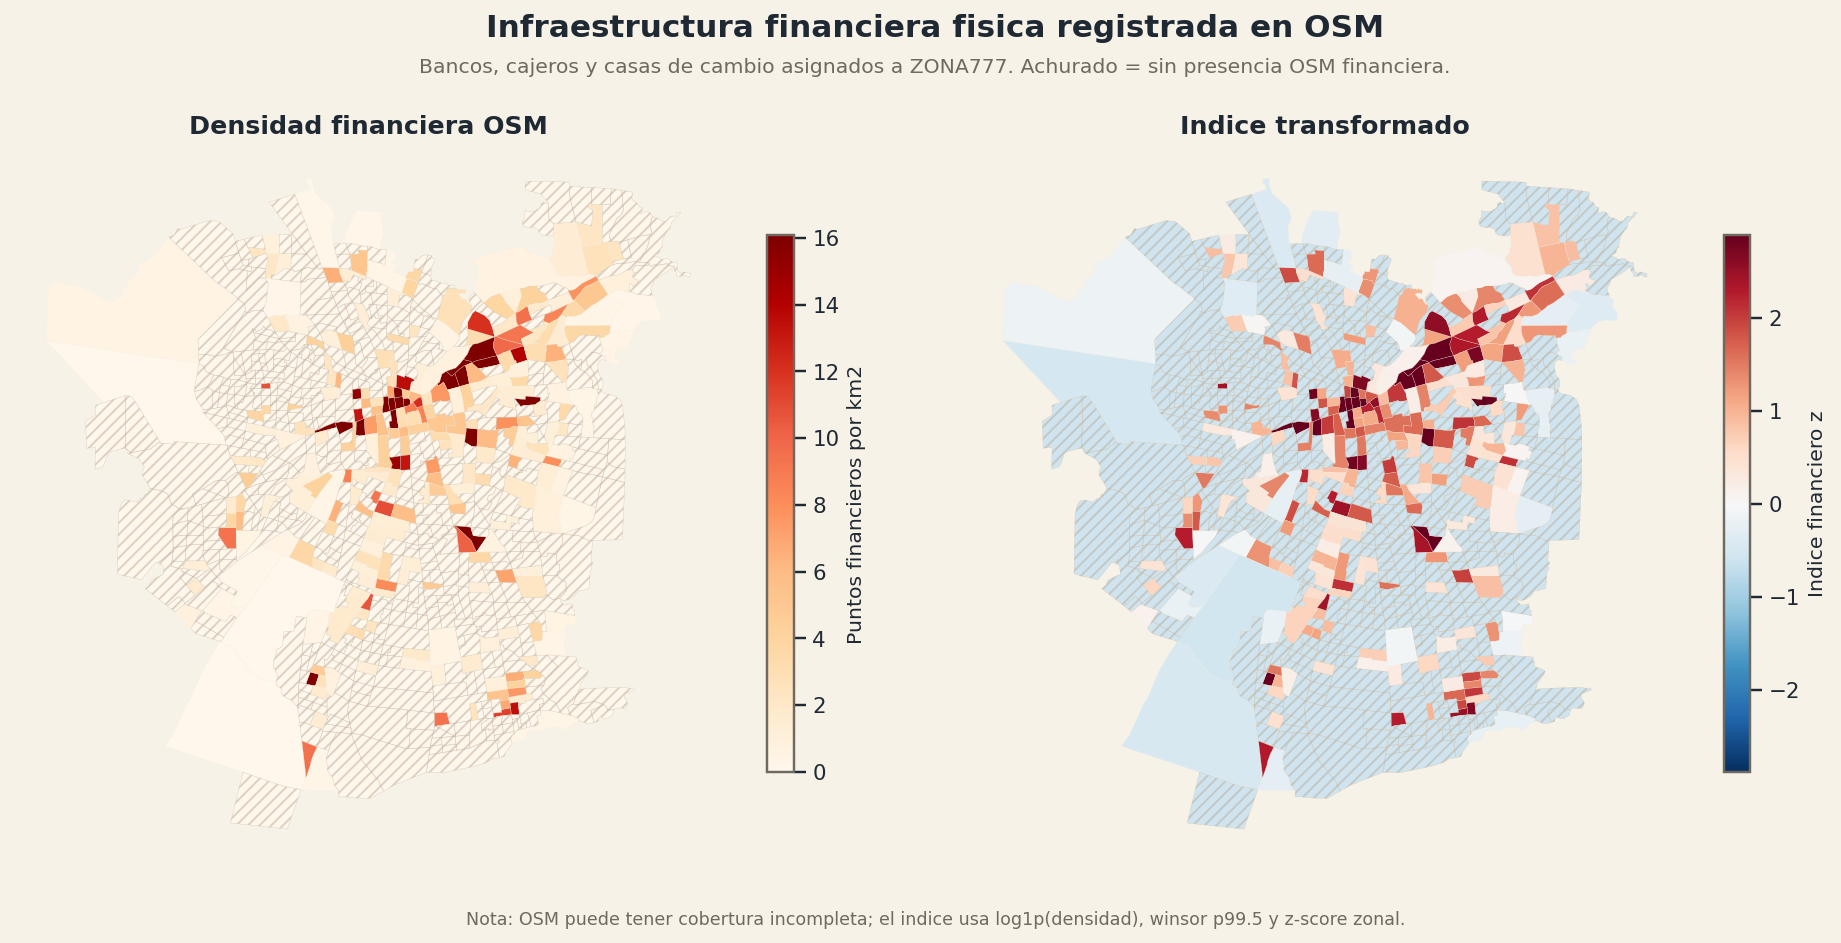
\includegraphics[width=0.94\textwidth]{block11-osm-financial-zone-map.png}
\caption{Infraestructura financiera física registrada en OSM}
\end{figure}

La infraestructura financiera OSM agrupa bancos, cajeros automáticos y casas de
cambio. Su distribución es claramente central: concentra valores altos en zonas
centrales y ejes de actividad, y valores bajos o nulos en muchas zonas
periféricas. Por eso, más que medir ``bancarización'', esta variable captura un
contexto territorial de centralidad y servicios financieros físicos.

\begin{figure}[H]
\centering
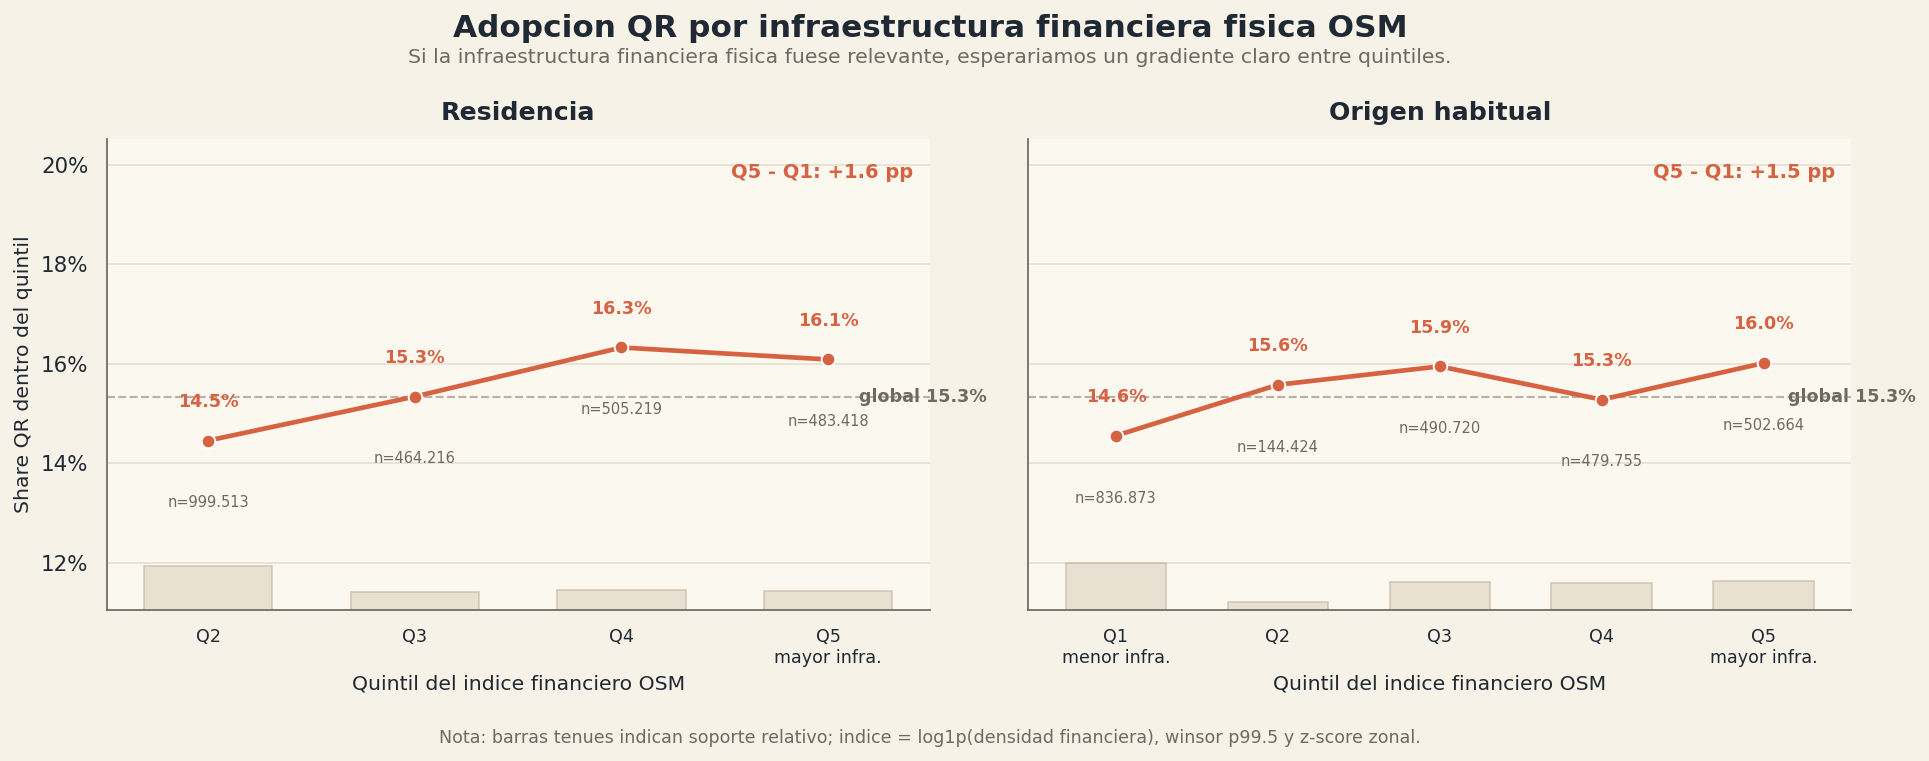
\includegraphics[width=0.88\textwidth]{block11-osm-financial-quintiles.png}
\caption{Adopción QR por intensidad de infraestructura financiera OSM}
\end{figure}

El gradiente es positivo pero moderado. En residencia, el share QR sube en torno
a 1.6 puntos porcentuales entre el quintil de menor y mayor intensidad
financiera OSM; en origen habitual, la diferencia es similar. La lectura
defendible es contextual: QR pesa algo más en zonas con mayor infraestructura
financiera física, pero la variable está mezclada con centralidad, ingreso,
educación y macrozona.

\begin{figure}[H]
\centering
\includegraphics[width=0.94\textwidth]{block12d-osm-commerce-map-output-2.png}
\caption{Comercio y servicios cotidianos registrados en OSM}
\end{figure}

El índice de comercio y servicios cotidianos incluye \texttt{shop=*} y
amenities de consumo diario, como restaurantes, cafés, comida rápida, bares,
mercados y farmacias. No incluye \texttt{office=*}, para no confundir comercio
local con actividad laboral u oficinas. Igual que el índice financiero, describe
centralidad urbana y mezcla de usos, no consumo individual.

\begin{figure}[H]
\centering
\includegraphics[width=0.90\textwidth]{block12d-osm-commerce-quintile-plot-output-2.png}
\caption{Adopción QR por densidad de comercio y servicios OSM}
\end{figure}

La señal de comercio/servicios también es positiva, aunque no perfectamente
monótona. En residencia, QR pasa de 14.1\% en el quintil de menor intensidad a
17.1\% en el mayor; en origen habitual, el patrón es más irregular pero los
quintiles altos quedan por sobre los bajos. Esto refuerza la idea de que QR se
asocia a contextos urbanos más centrales, no a un mecanismo aislado de comercio
local.

\subsection{Equipamientos urbanos OSM no comerciales}

El bloque de equipamientos OSM separa componentes en vez de construir un único
índice agregado. Se revisan escuelas, educación superior, salud general, centros
cívicos o comunitarios, parques, juegos infantiles y equipamiento deportivo
barrial. Cada componente tiene una geografía distinta, por lo que hablar de
``equipamiento'' sin apellido sería ambiguo.

\begin{figure}[H]
\centering
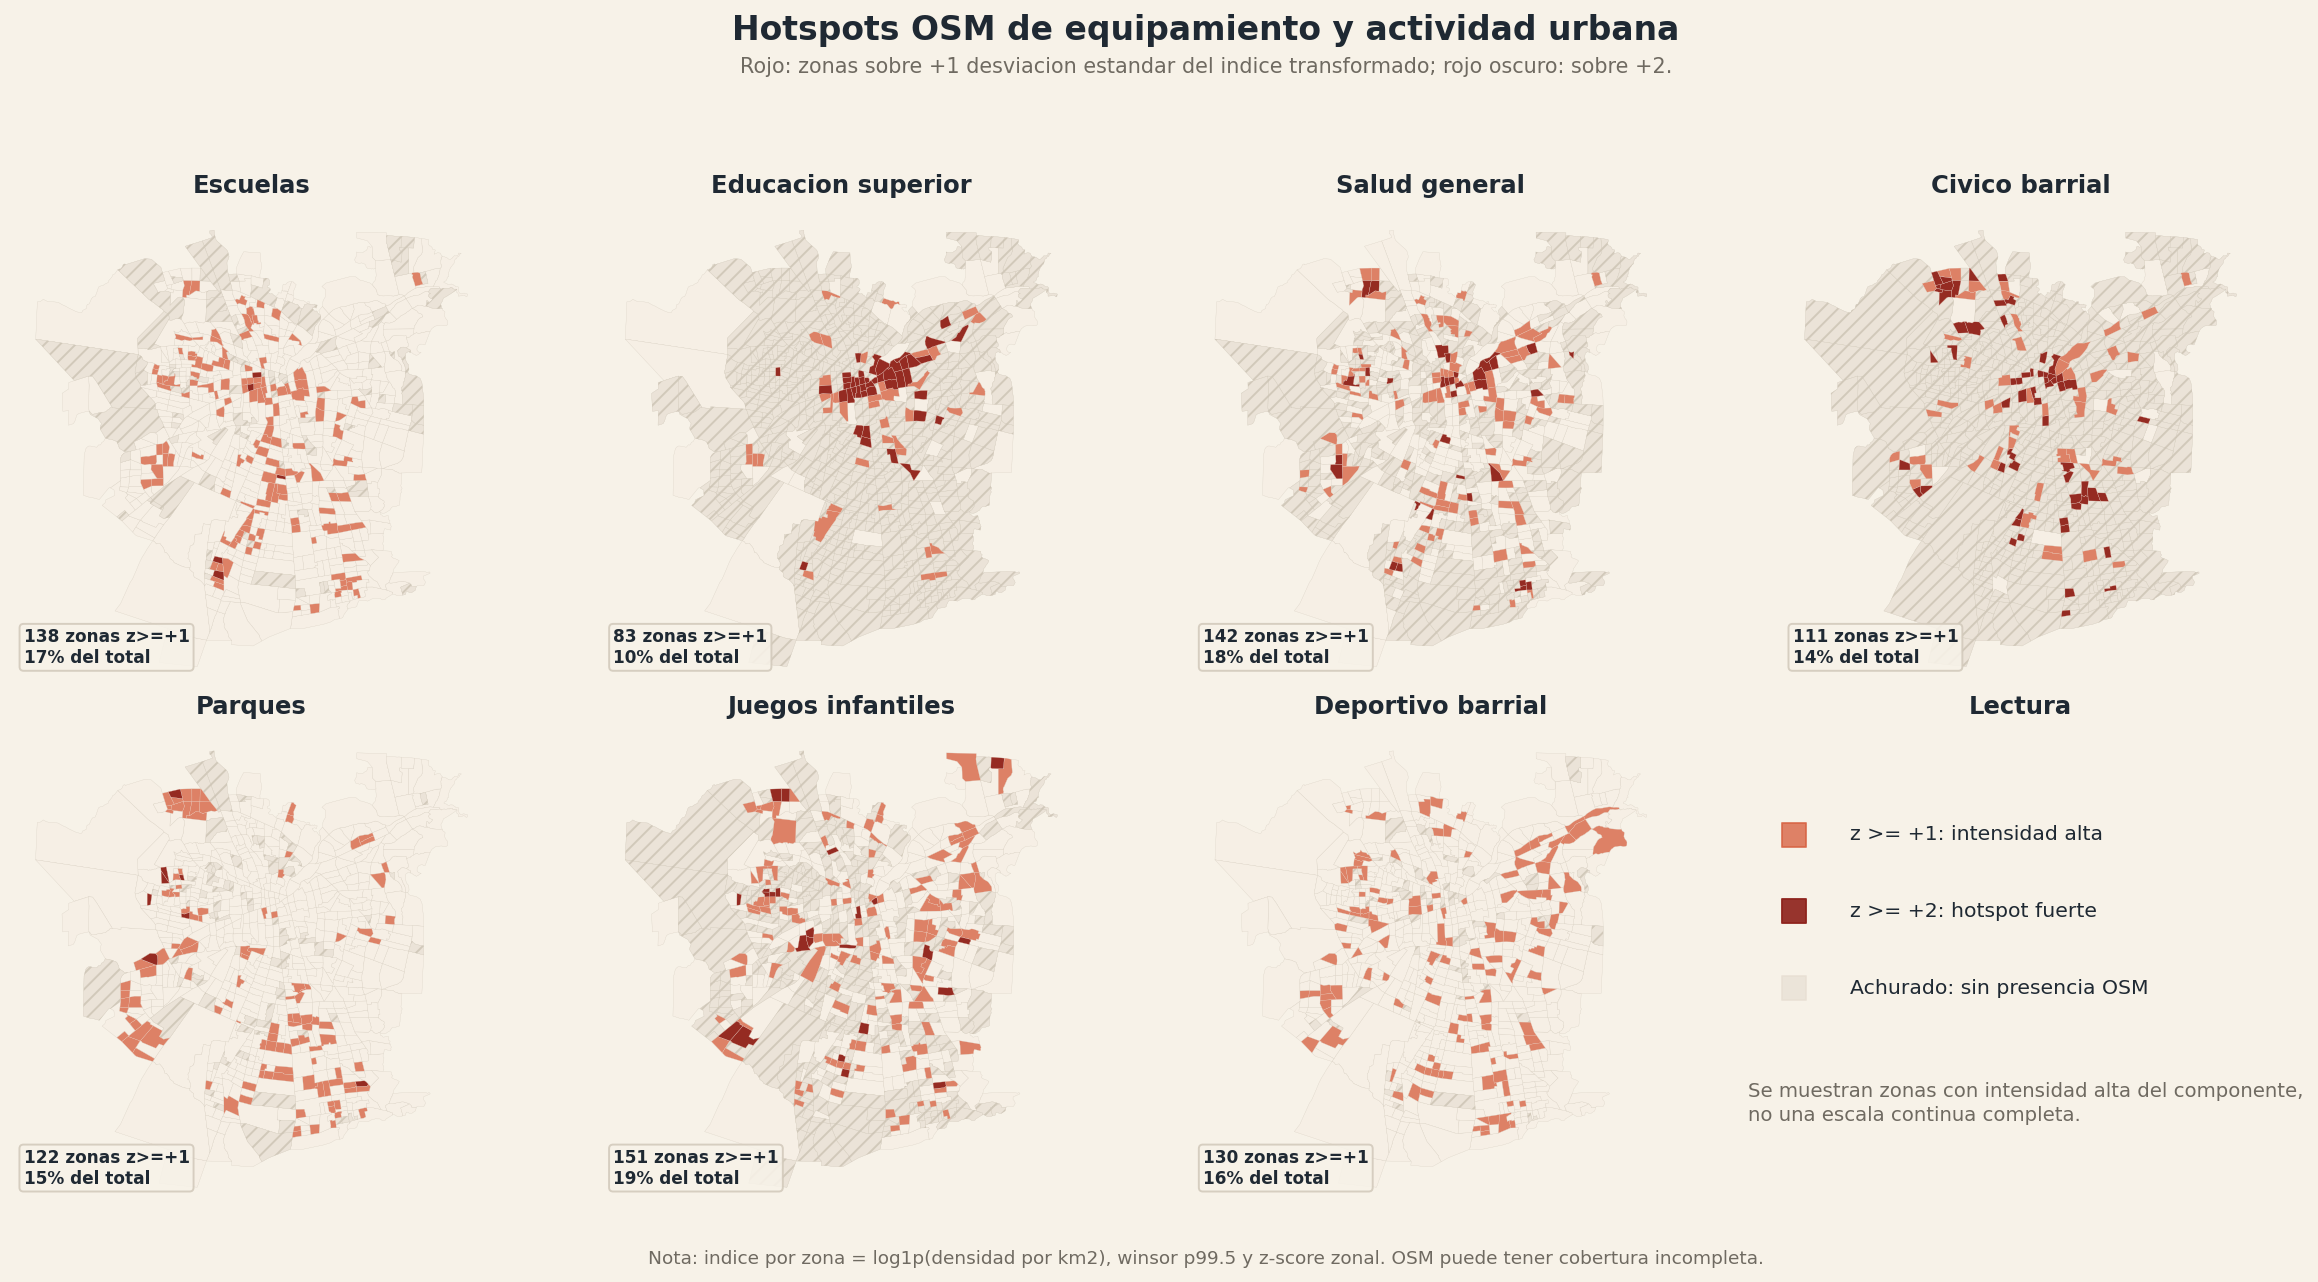
\includegraphics[width=0.98\textwidth]{block12f-osm-activity-hotspots.png}
\caption{Hotspots OSM de equipamientos urbanos no comerciales}
\end{figure}

El mapa no compara QR contra BIP. Su función es mostrar dónde se concentran los
distintos tipos de objetos urbanos registrados en OSM. Educación superior y
centros cívicos se concentran en centralidades específicas; escuelas, salud,
juegos infantiles y equipamiento deportivo aparecen más dispersos. Las zonas
achuradas no tienen presencia registrada del componente.

\begin{figure}[H]
\centering
\includegraphics[width=0.90\textwidth]{block12f-osm-activity-qrbip-profile-output-3.png}
\caption{Diferencia QR--BIP en componentes de equipamiento urbano OSM}
\end{figure}

La comparación QR--BIP muestra diferencias pequeñas. En residencia, la mayor
distancia favorable a QR aparece en salud general, cerca de +0.10 desviaciones
estándar del índice zonal. En origen habitual, salud general y juegos infantiles
también quedan algo por sobre BIP, pero alrededor de una décima de desviación
estándar. Educación superior y centros cívicos son territorialmente
concentrados, pero no separan a QR y BIP en la mediana heredada.

\subsection{Oferta, demanda y relación demanda-oferta operacional}

Las variables operacionales se reconstruyen desde viajes observados, frecuencias
bus y oferta programada Metro. En bus, oferta refiere a paraderos activos o
pasadas programadas; demanda refiere a subidas observadas; y la relación
demanda-oferta se calcula como subidas observadas por pasada bus programada en
la misma celda paradero-hora. En Metro, oferta se aproxima con estaciones,
líneas o trenes programados; demanda refiere a validaciones de ingreso de
pasajeros al Metro en una estación y hora observada; y la relación
demanda-oferta se calcula como validaciones observadas por pasada
tren-estación programada. Cuando el texto usa ``presión'', se refiere solo a
esta razón demanda/oferta. No mide ocupación dentro del bus o tren, espera real,
calidad de servicio ni causalidad.

Para comparar semanas y franjas horarias, las variables se transforman a
percentiles dentro de cada semana-franja y luego se promedian sobre los viajes
de cada tarjeta. Por eso, un valor alto significa que la tarjeta observa
contextos operacionales relativamente altos dentro de su semana y franja, no un
número bruto comparable entre toda la ciudad.

\begin{figure}[H]
\centering
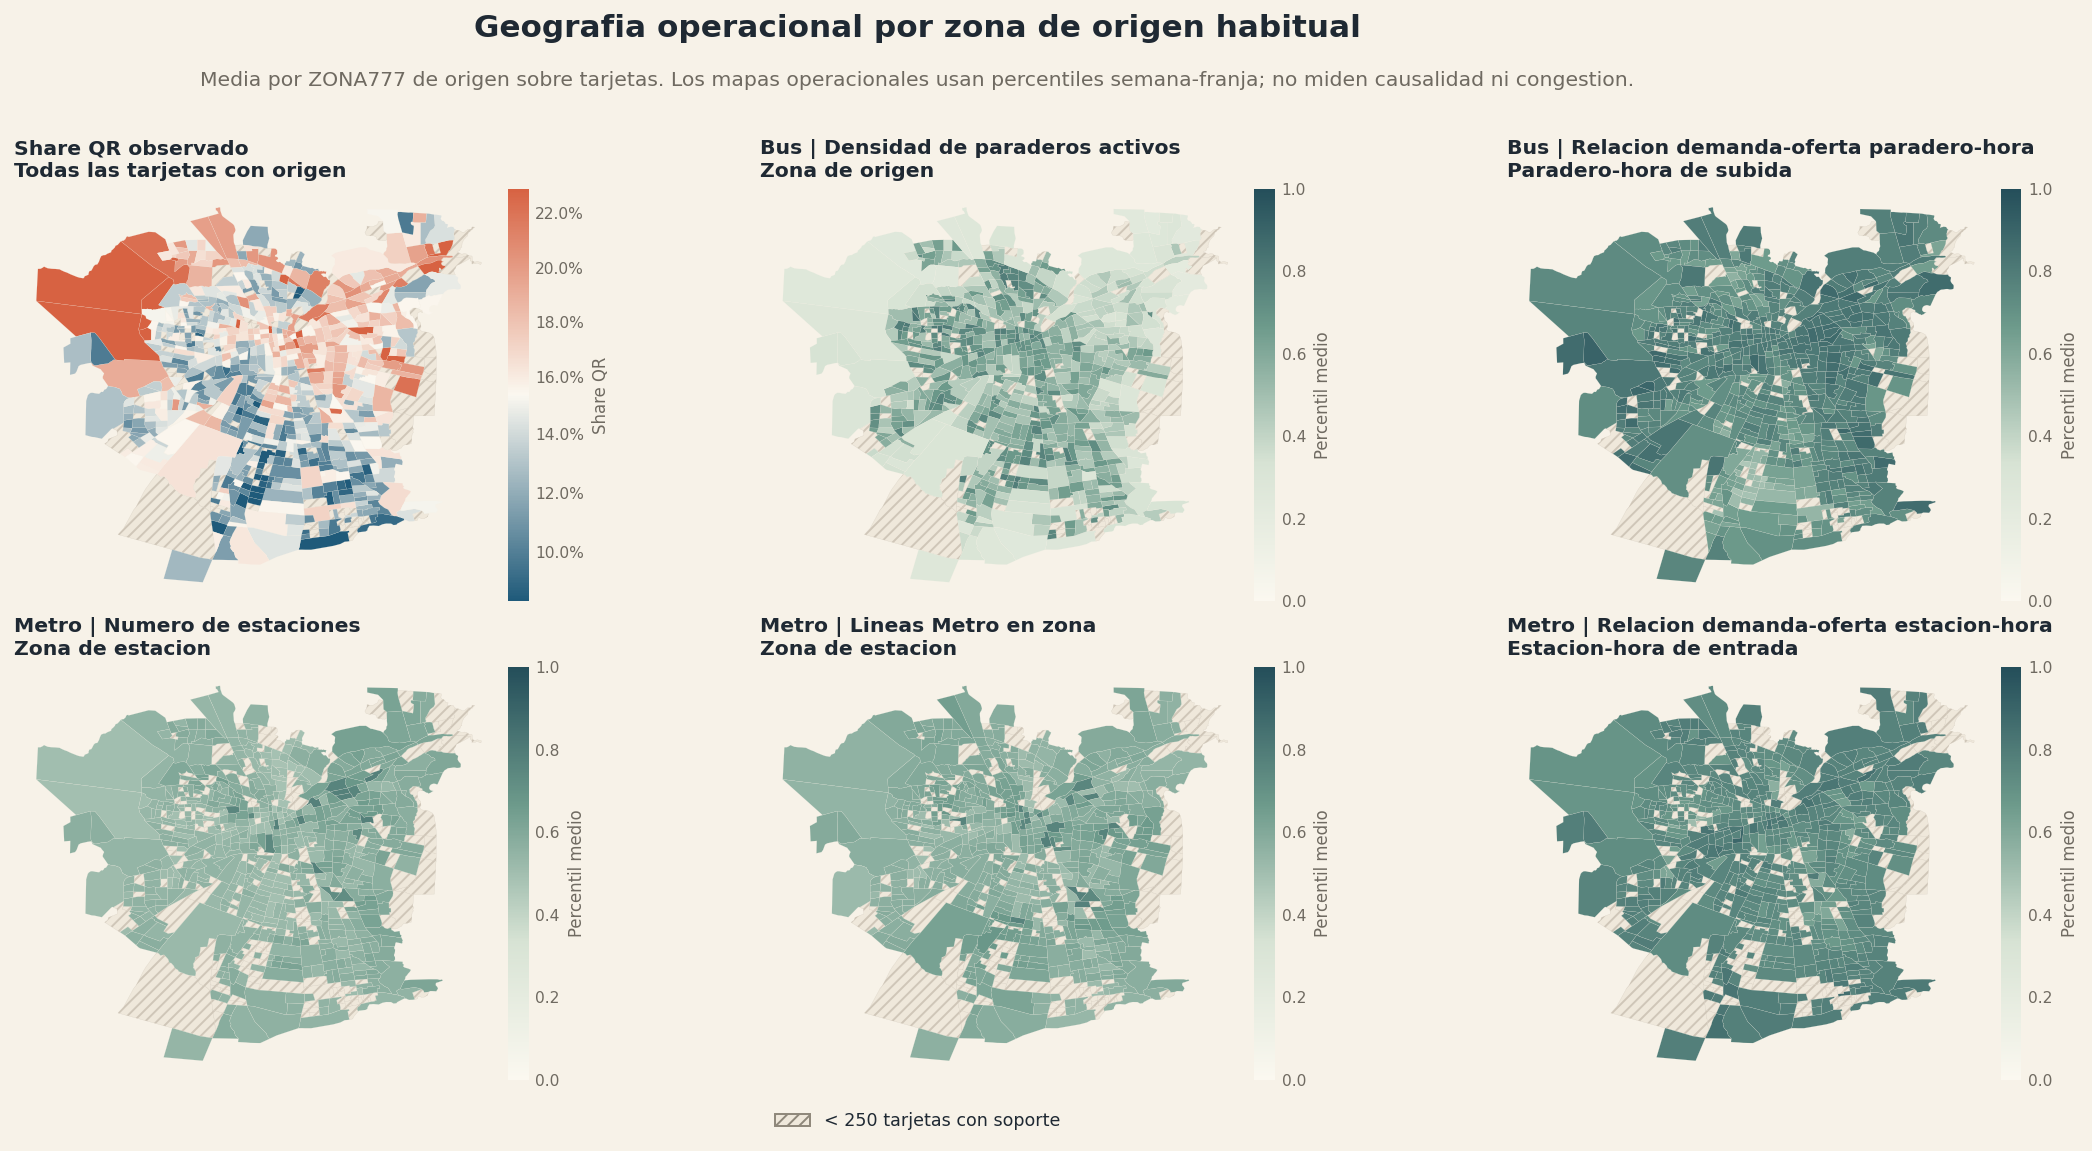
\includegraphics[width=0.96\textwidth]{block13-operational-origin-zone-map.png}
\caption{Geografía operacional por zona de origen habitual}
\end{figure}

El mapa muestra que las variables operacionales también tienen geografía propia.
La presencia Metro, la densidad de paraderos activos y las relaciones
demanda-oferta bus/Metro no se distribuyen igual en la ciudad. Esto importa
porque cualquier diferencia QR/BIP en operación puede mezclar condiciones del
sistema con centralidad territorial y perfil de usuarios.

\begin{figure}[H]
\centering
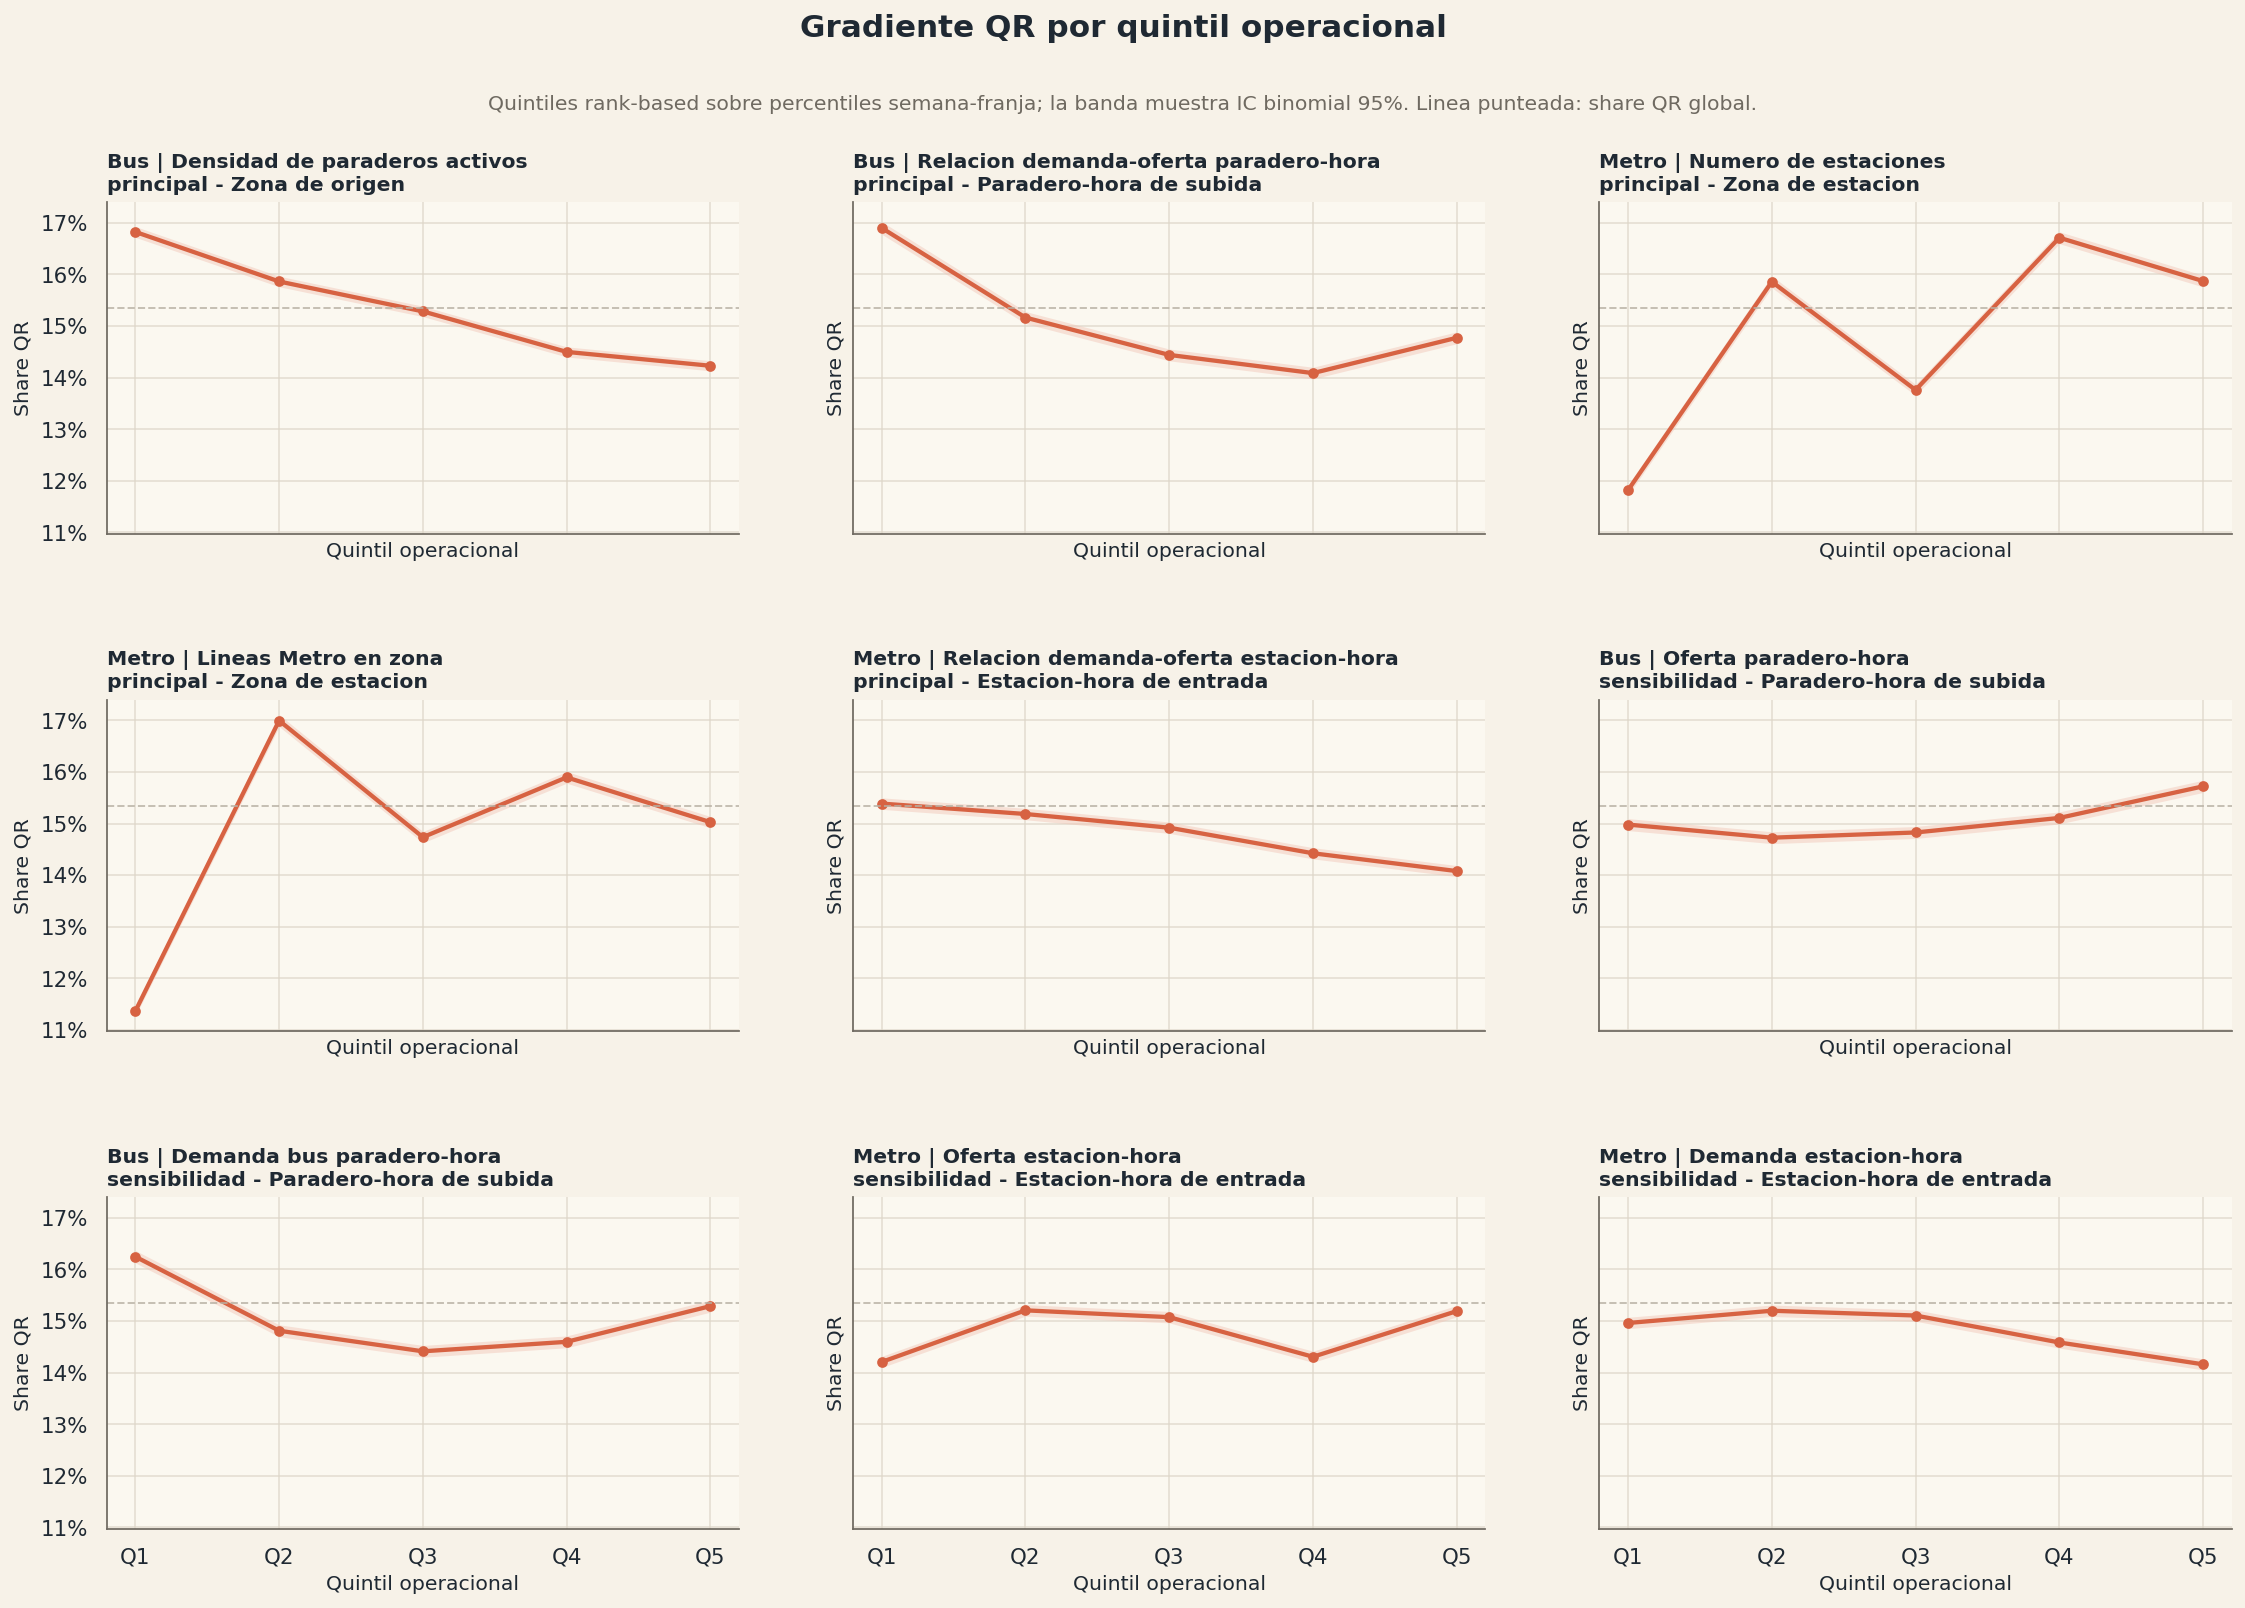
\includegraphics[width=0.96\textwidth]{block13-operational-qr-quintile-gradients.png}
\caption{Adopción QR por quintil de variables operacionales}
\end{figure}

La lectura operacional no es ``más oferta, más QR''. En bus, QR tiende a pesar
menos en contextos de mayor densidad de paraderos y mayor relación
demanda-oferta. En Metro aparece una señal distinta: QR pesa más en zonas con
mayor presencia de estaciones o líneas, aunque la relación demanda-oferta Metro
no muestra una señal positiva clara. En síntesis, las variables operacionales
describen contexto de origen habitual: QR se asocia menos a entornos bus densos
o presionados y algo más a presencia Metro, sin que esto implique causalidad.

\paragraph{Cierre del bloque.}
El contexto urbano y operacional refuerza una lectura de centralidad, no de
escasez de alternativas BIP ni de presión operacional como mecanismo principal.
Los indicadores OSM muestran que QR hereda zonas algo más centrales y con más
infraestructura registrada, especialmente financiera y comercial, pero los
equipamientos urbanos no comerciales separan poco a QR y BIP. En operación, la
señal más consistente es presencia Metro; las relaciones demanda-oferta de bus y
Metro no apuntan a que QR se concentre donde el sistema está más exigido. Este
bloque, por tanto, sirve para caracterizar el entorno territorial de QR, no para
atribuir causalidad a una variable aislada.

\section{Cambio interanual 2024--2025}

El bloque interanual pregunta si el aumento QR entre 2024 y 2025 fue homogéneo
o si algunas zonas crecieron más que la tendencia global. La comparación usa
ventanas equivalentes de cuatro semanas: \texttt{2024-W14} a \texttt{2024-W17}
y \texttt{2025-W14} a \texttt{2025-W17}. Por eso, no es un balance anual
completo, sino una comparación controlada por semana calendario.

Se usan dos geografías. En residencia, la unidad es tarjeta-año clasificada
como QR o BIP y agrupada por \texttt{zona\_hogar}. En origen de viaje, la
unidad es viaje iniciado en la zona. En ambos casos, el cambio zonal se define
como:
\[
\Delta_z = \text{share QR}_{z,2025} - \text{share QR}_{z,2024}.
\]
Cuando se habla de crecimiento relativo, se descuenta el cambio global de la
misma geografía:
\[
\Delta^{rel}_z = \Delta_z - \Delta_{global}.
\]
Así, un valor positivo no significa solo que QR subió, sino que subió más que la
tendencia global de su geografía.

\begin{figure}[H]
\centering
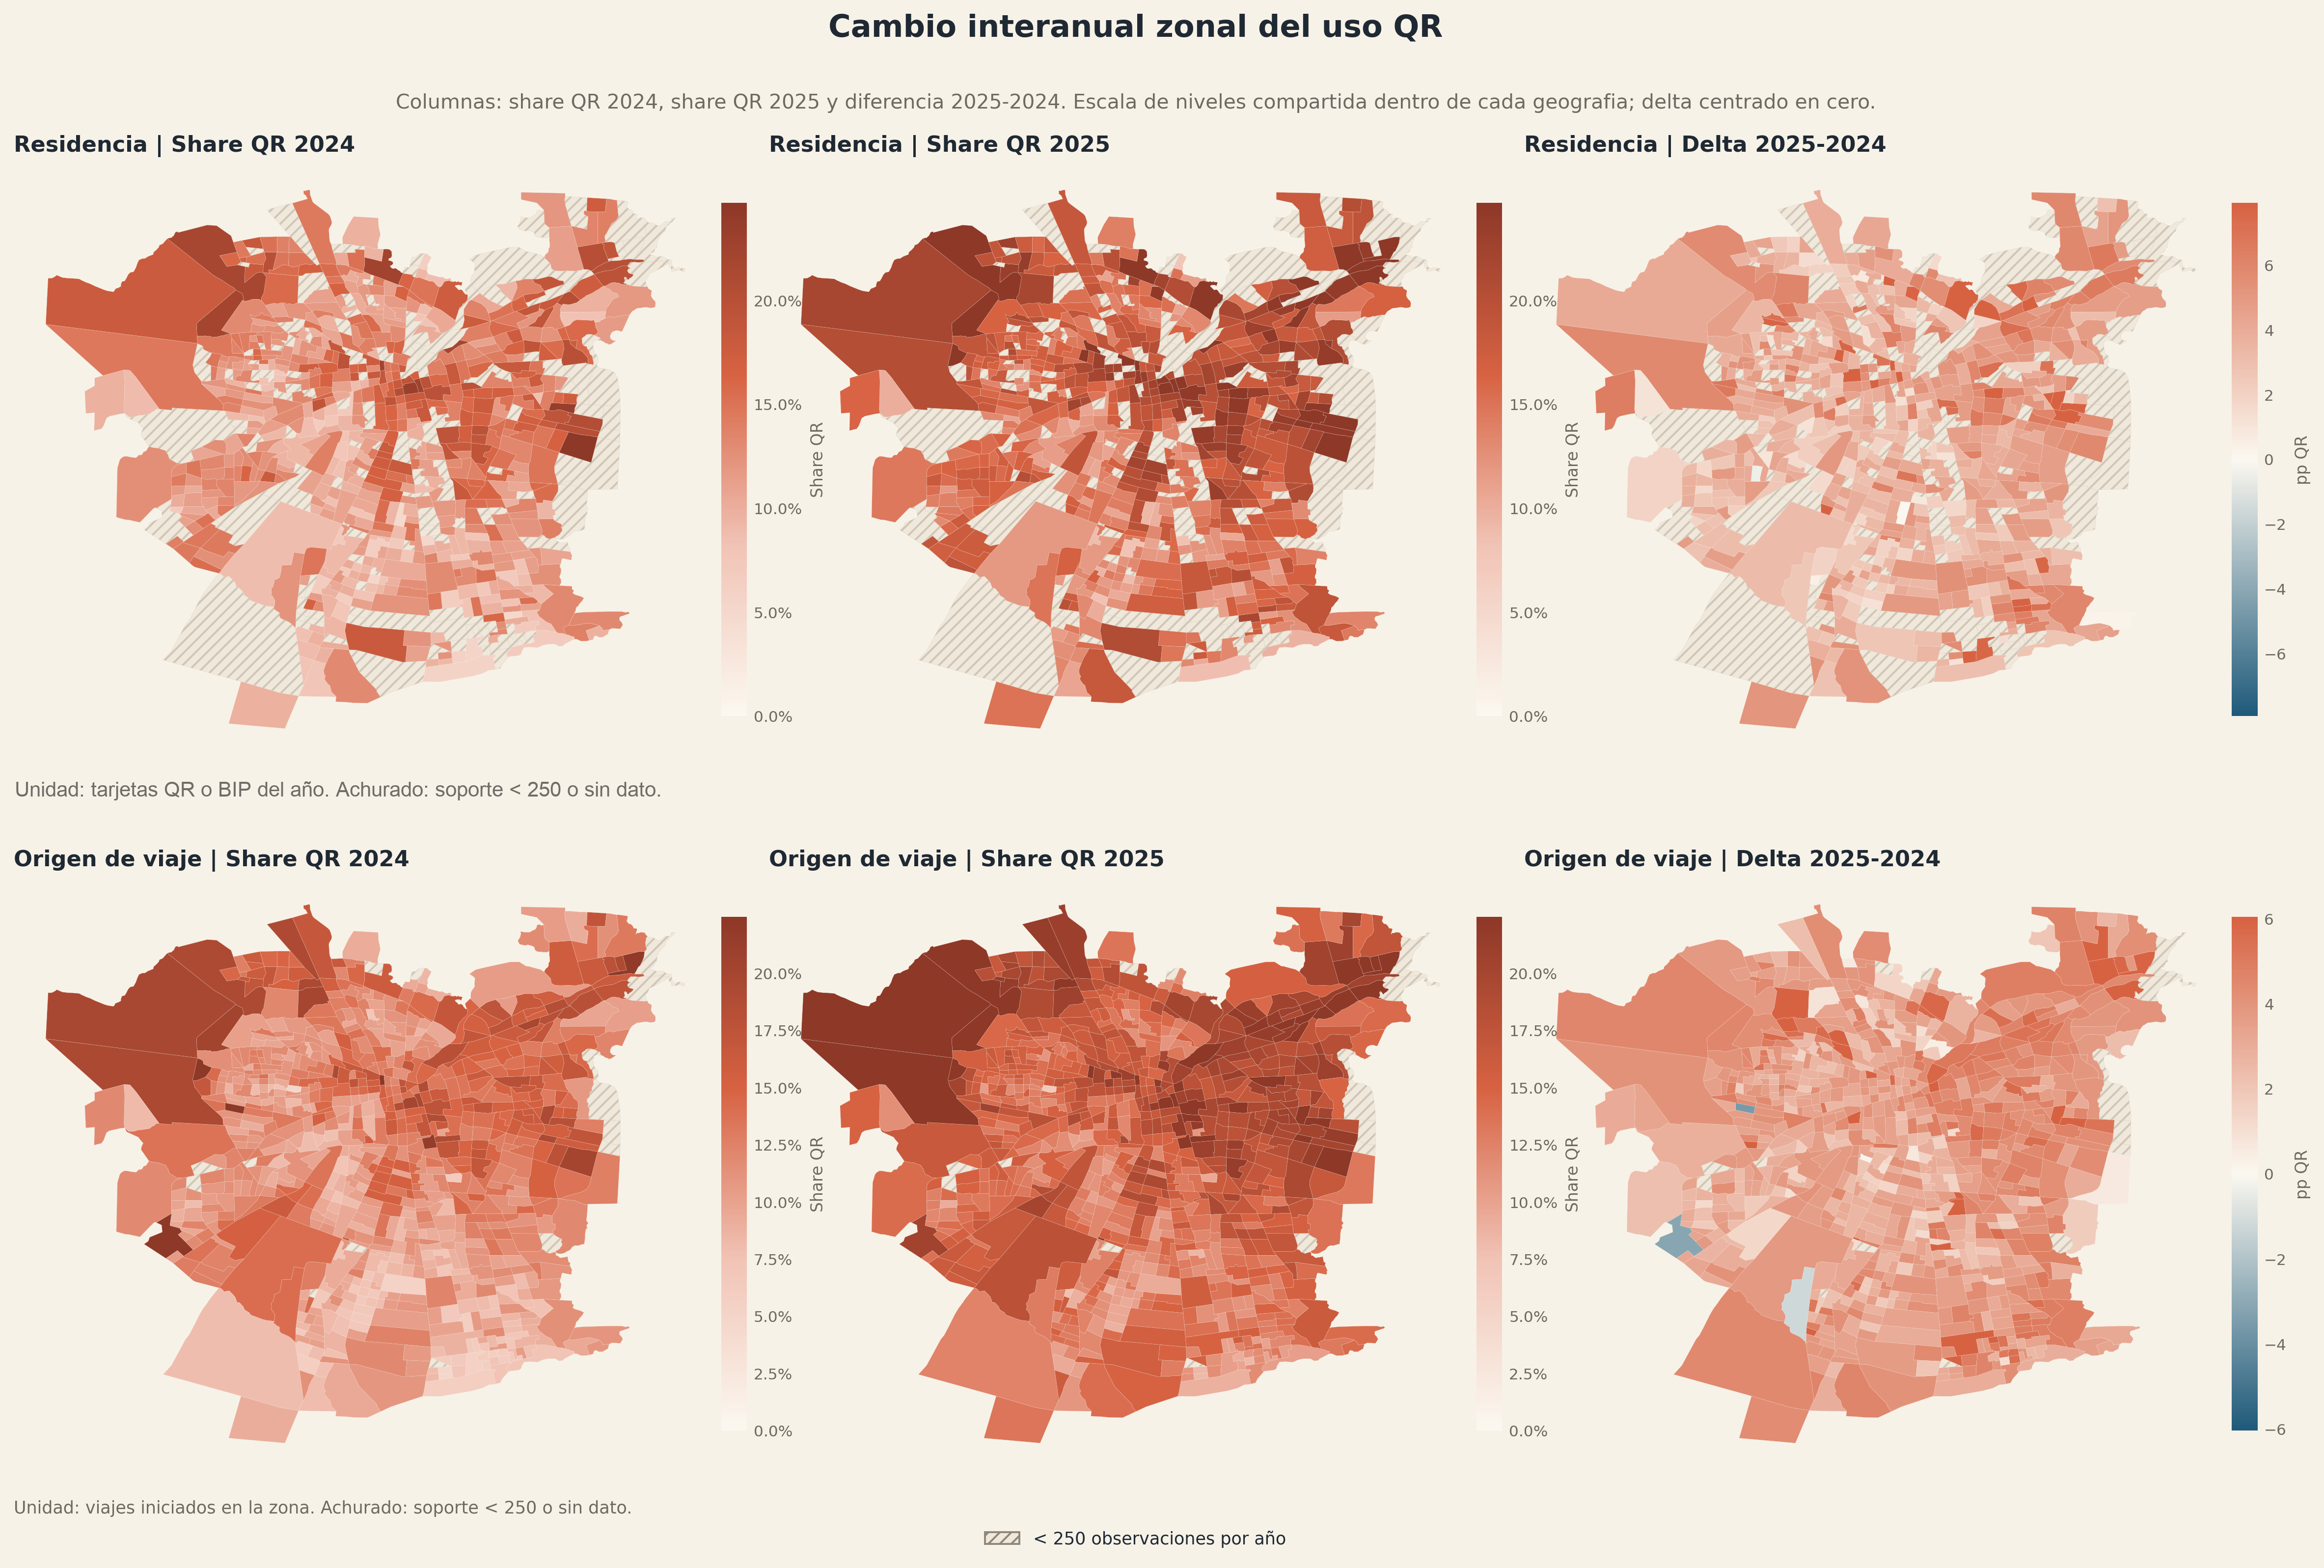
\includegraphics[width=0.98\textwidth]{block14a-interannual-zone-change-maps-corrected.png}
\caption{Cambio interanual zonal del uso QR}
\end{figure}

La primera lectura es de expansión generalizada. En residencia, el share QR sube
de 13.9\% en 2024 a 18.1\% en 2025, con un aumento global de +4.22 puntos
porcentuales. En origen de viaje, sube de 12.8\% a 16.8\%, con un aumento de
+3.96 puntos porcentuales. Casi todas las zonas con soporte comparable aumentan
su share QR: 99.7\% en residencia y 99.5\% en origen de viaje.

Esto cambia la pregunta sustantiva. El fenómeno no es que QR aparezca solo en
algunas zonas aisladas, sino que crece casi en toda la ciudad. Lo relevante pasa
a ser dónde crece más o menos que la tendencia global.

\begin{figure}[H]
\centering
\includegraphics[width=0.98\textwidth]{block14b-interannual-persistence-relative-growth-output-4.png}
\caption{Persistencia espacial y crecimiento relativo QR}
\end{figure}

La geografía QR es muy persistente. La correlación ponderada entre share QR
zonal 2024 y 2025 es 0.96 en residencia y 0.97 en origen de viaje. Las zonas
que ya tenían más QR en 2024 tienden a seguir arriba en 2025.

Además, hay una señal de refuerzo territorial. El nivel QR inicial se asocia
positivamente con el crecimiento relativo: +0.27 en residencia y +0.44 en
origen de viaje. En términos simples, varias zonas que ya partían con mayor QR
también crecieron más que el promedio global. Esto no implica que todas las
zonas altas sean top de crecimiento, pero sí sugiere persistencia con cierto
refuerzo.

\subsection{Variables candidatas del crecimiento relativo}

El cruce con variables candidatas es descriptivo. No estima un modelo ni
atribuye causalidad; solo muestra qué atributos zonales se alinean con el
crecimiento relativo QR.

\begin{figure}[H]
\centering
\includegraphics[width=0.98\textwidth]{block14f-interannual-candidate-scatter-diagnostics-output-3.png}
\caption{Variables candidatas y crecimiento relativo QR zona a zona}
\end{figure}

En residencia, el crecimiento relativo QR es mayor en zonas con más educación
universitaria+ residencial y menor en zonas con mayor concentración D+E. La
educación universitaria+ es la señal residencial más consistente del screening:
correlación Spearman con delta de +0.30, correlación parcial controlando share
QR 2024 de +0.23 y diferencia Q5--Q1 de +1.33 puntos porcentuales. La
concentración D+E va en sentido opuesto.

Las variables OSM de centralidad urbana, como comercio/servicios e
infraestructura financiera, muestran señales positivas pero moderadas. En origen
de viaje, las variables operacionales más informativas son presencia Metro y
demanda bus. En cambio, el acceso físico a carga BIP mantiene señal débil: no
aparece como explicación dominante del crecimiento interanual QR.

\subsection{Tipología territorial y aporte volumétrico}

La tipología clasifica zonas según crecimiento relativo: top 20\% si crecen más
que la tendencia global, bottom 20\% si crecen menos y middle 60\% si quedan
cerca de la tendencia. El mapa no muestra nivel absoluto QR; muestra posición
relativa de crecimiento.

\begin{figure}[H]
\centering
\includegraphics[width=0.98\textwidth]{block14g-interannual-relative-growth-typology-map-output-3.png}
\caption{Tipología territorial del crecimiento relativo QR}
\end{figure}

La tipología muestra focos de alto crecimiento relativo, pero también muchos
espacios intermedios. En residencia, Oriente concentra una fracción alta de
zonas top, mientras Sur y Poniente aparecen con más zonas bottom. En origen de
viaje, Oriente vuelve a destacar, pero también aparecen focos en Suroriente y
algunas zonas periféricas. Esta figura sirve para ubicar el patrón espacial, no
para medir cuánto aporta cada zona al aumento agregado.

\clearpage

\begin{figure}[H]
\centering
\includegraphics[width=0.98\textwidth]{block14i-interannual-volume-contribution-output-4.png}
\caption{Contribución volumétrica al aumento QR por macrozona}
\end{figure}

La contribución por volumen cambia parte de la lectura. Se calcula como
\[
\text{observaciones 2025} \times
(\text{share QR}_{2025} - \text{share QR}_{2024}),
\]
manteniendo fijo el volumen 2025. En residencia, el mayor aporte al aumento QR
proviene de Poniente (25.6\%), Suroriente (20.6\%) y Oriente (18.8\%). En origen
de viaje, el mayor aporte proviene de Oriente (29.8\%), Centro (18.7\%),
Poniente (18.3\%) y Suroriente (17.2\%).

Esto distingue crecimiento relativo de peso agregado. Oriente aparece fuerte en
crecimiento relativo, pero en residencia Poniente aporta más al aumento agregado
por su volumen. En origen de viaje, Oriente sí combina ambas cosas: alto
crecimiento relativo y gran contribución volumétrica.

\paragraph{Cierre del bloque.}
El bloque interanual muestra que QR crece de forma amplia entre ventanas
equivalentes de 2024 y 2025, pero sin borrar la geografía previa. La estructura
territorial se mantiene y, en parte, se refuerza. Las señales que mejor
acompañan el crecimiento relativo son educación residencial, menor
concentración D+E, centralidad urbana y presencia operacional Metro/bus. El
acceso físico a carga BIP no aparece como mecanismo dominante. Esta lectura deja
planteado un segundo paso natural: un modelo zonal de crecimiento QR que controle
por share inicial, volumen, macrozona y familias de variables territoriales.

\clearpage

\section{Cierre}

\paragraph{Qué sabemos.}
QR sigue siendo minoritario frente a BIP, pero ya tiene una presencia suficiente
para estudiar patrones territoriales y temporales. Su uso aparece menos intensivo
por tarjeta, sin que eso implique una separación limpia entre usuarios QR y BIP:
las distribuciones se solapan y las diferencias son agregadas. Territorialmente,
QR se asocia más a zonas de mayor centralidad, mayor educación residencial, mayor
ingreso residencial y mayor presencia operacional Metro/bus. Entre 2024 y 2025,
QR crece de forma amplia, casi en todas las zonas comparables, pero el crecimiento
no es homogéneo: la geografía previa persiste y algunas zonas crecen más que la
tendencia global.

\paragraph{Qué no podemos afirmar.}
Este EDA no permite decir que esas variables causan adopción QR, ni que las
tarjetas QR pertenezcan individualmente a personas de mayor ingreso o educación.
Las variables residenciales, OSM y operacionales son atributos heredados desde
zonas; describen contexto territorial, no características personales. Tampoco se
observa una conversión individual BIP a QR, ni se mide calidad de infraestructura,
tiempos de espera, congestión real o acceso efectivo a medios de pago. Por eso,
las diferencias deben leerse como patrones descriptivos de zonas y tarjetas, no
como mecanismos identificados.

\paragraph{Qué habilita.}
La hipótesis de trabajo más defendible es zonal, no individual: el crecimiento QR
parece alinearse con centralidad urbana, composición socioeconómica residencial y
conectividad operacional, más que con falta de acceso físico a carga BIP. Un
siguiente EDA o modelo puede evaluar si estas familias de variables siguen
aportando señal al explicar el aumento QR 2025--2024 después de controlar por el
share QR inicial, el volumen observado, la macrozona y la dependencia entre
variables territoriales. Esa sería una forma natural de pasar desde lectura
descriptiva hacia un modelo zonal de crecimiento.

\end{document}
